%%%%%%%%%%%%%%%%%%%%%%%%%%%%%%%%%%%%%%%%%
% Thin Sectioned Essay
% LaTeX Template
% Version 1.0 (3/8/13)
%
% This template has been downloaded from:
% http://www.LaTeXTemplates.com
%
% Original Author:
% Nicolas Diaz (nsdiaz@uc.cl) with extensive modifications by:
% Vel (vel@latextemplates.com)
%
% License:
% CC BY-NC-SA 3.0 (http://creativecommons.org/licenses/by-nc-sa/3.0/)
%
%%%%%%%%%%%%%%%%%%%%%%%%%%%%%%%%%%%%%%%%%

%----------------------------------------------------------------------------------------
%	PACKAGES AND OTHER DOCUMENT CONFIGURATIONS
%----------------------------------------------------------------------------------------

\documentclass[a4paper, 12pt]{article} % Font size (can be 10pt, 11pt or 12pt) and paper size (remove a4paper for US letter paper)

\usepackage[protrusion=true,expansion=true]{microtype} % Better typography
\usepackage[frenchb]{babel}
\usepackage{graphicx} % Required for including pictures
\usepackage{wrapfig} % Allows in-line images

\usepackage{mathpazo} % Use the Palatino font
\usepackage[utf8]{inputenc} % UTF-8 encoding for input, to get french special characters recognized
\usepackage[T1]{fontenc} % Required for accented characters
\linespread{1.05} % Change line spacing here, Palatino benefits from a slight increase by default
\usepackage{parskip} % add some space between paragraph 
 
\makeatletter
\renewcommand\@biblabel[1]{\textbf{#1.}} % Change the square brackets for each bibliography item from '[1]' to '1.'
\renewcommand{\@listI}{\itemsep=0pt} % Reduce the space between items in the itemize and enumerate environments and the bibliography

\renewcommand{\maketitle}{ % Customize the title - do not edit title and author name here, see the TITLE block below
\begin{flushright} % Right align
{\LARGE\@title} % Increase the font size of the title

\vspace{50pt} % Some vertical space between the title and author name

{\large\@author} % Author name
%\\\@date % Date

\vspace{40pt} % Some vertical space between the author block and abstract
\end{flushright}
}

%----------------------------------------------------------------------------------------
%	TITLE
%----------------------------------------------------------------------------------------

%\title{\textbf{Techniques d'optimisation des temps de chargements dans les jeux à monde ouvert}\\ % Title
%Ou comment réduire les temps de chargement} % Subtitle
%
%\author{\textsc{Christian NGO \& Jonathan MULLER} % Author
%\\{\textit{ESGI - 5ème année IJV}}} % Institution
%
%\date{\today} % Date 

%----------------------------------------------------------------------------------------

\begin{document}

%\maketitle % Print the title section

%----------------------------------------------------------------------------------------
%	ABSTRACT AND KEYWORDS
%----------------------------------------------------------------------------------------

%\renewcommand{\abstractname}{Summary} % Uncomment to change the name of the abstract to something else

%\begin{abstract}
%Dans ce mémoire nous verrons comment réduire les temps de chargement des jeux vidéos en se basant à la fois sur les composants de la plate-forme cible, sur les techniques de compression, sur l'algorithme et sur le level design.
%\end{abstract}
%
%\hspace*{3,6mm}\textit{Mots clefs:} chargement , optimisation , ressources , streaming , jeu % Keywords
%
%\vspace{30pt} % Some vertical space between the abstract and first section

%----------------------------------------------------------------------------------------
%	ESSAY BODY
%----------------------------------------------------------------------------------------

\tableofcontents
\newpage
\section{Avant-propos}
\subsection{Remerciements}
Nous tenons à remercier:

M. Nicolas VIDAL, notre maître de mémoire pour nous avoir guidé dans notre travail ainsi que pour son soutien. Il a su nous orienter lors de nos choix et de nos recherches.

M. Emmanuel PETER, pour la mise à disposition des locaux et du matériel, ainsi que la selection des cours de qualité dispensés à l'ESGI qui nous ont permis d'acquérir les connaissances nécessaires pour nos recherches.

L'équipe pédagogique de l'ESGI, pour sa réactivité et les réponses claires à nos questions concernant le mémoire.


\newpage

\subsection{Résumé}
Depuis leur création, les jeux vidéo ne cessent d'évoluer à tous les niveaux : univers, gameplay, graphismes, techniques de développement, ressources, etc. De nos jours, les jeux vidéo sont de plus en plus gourmands en terme de volume et de ressources matériels requis. Ceci est dû à une volonté de rendre ces jeux plus réalistes et plus jolis pour en mettre plein la vue. Il faut pour cela, créer des ressources (éléments du jeux tels que les personnages, objets, décors, etc.) de plus en plus détaillés, ce qui augmente considérablement leur poids. Ainsi il faut toujours plus d'espace sur les supports mais aussi plus d'espace mémoire allouée pour charger ces éléments et les afficher au cours d'une session de jeu. Les développeurs ont dû mettre en place des techniques permettant d'optimiser les temps de chargement de ces ressources. A travers ce mémoire, nous souhaitons présenter et expliquer les différentes techniques utilisées par les développeurs que ce soit lors de la conception du jeu ou bien lors de son utilisation. Le but est de fournir aux jeunes concepteurs de jeux vidéo une liste des techniques d'optimisation les plus efficaces pour des cas particulier ainsi que les choses à éviter pour mener à bien le développement de leur jeu.

\subsection{Abstract}
Video games are evolving at any points : world, gameplay, graphics, development techniques, resources, etc. Nowadays, video games are really big and require lot of hardware resources. This is due to a desire to make them more realistic with better graphics. To do so, developers need to create resources (elements of games like characters, objetcs, backgrounds, etc.) more detailed, which greatly increase the space needed to store them. It also needs more memory space allocated to load and display these elements in a game session. Developers had to develop techniques to optimize the loading time of these resources. We wish to present and explain the various techniques used by developers to design their games. The goal is to provide young video game designers a list of the most effective optimization techniques as well as things to avoid to complete the development of their game.

\subsection{Mots clés}
\begin{center}
	\begin{tabular}{|p{0.45\columnwidth}|p{0.45\columnwidth}|}
		\hline
		Mots clés & Key words\\
		\hline
		Chargement&Loading\\
		Optimisation&Optimization\\
		Compression&Compression\\
		Ressources&Resources\\
		Jeu&Game\\
		Monde ouvert&Open World\\
		Level Design&Level Design\\
		LOD&LOD\\
		Shaders&Shaders\\
		Matériel&Hardware\\
		Organisation&Organization\\
		Perception&Perception\\
		Temps&Time\\
		\hline
	\end{tabular}
\end{center}

\newpage

\section{Introduction}
Les jeux vidéo comportent année après année un nombre grandissant de ressources nécessaires pour leur fonctionnement. Des textures aux modèles 3D, le poids de ces ressources augmente tout comme leur nombre, l'augmentation de la taille mémoire des machines permettant aux créateurs de jeux de charger plus de ressources à la fois. Cependant, augmenter la taille et le nombre des ressources a un prix, celui du temps de chargement. Dans ce mémoire nous verrons comment réduire ces temps de chargement en s'adaptant aux médias qui permettent de stocker les ressources du jeu, en tirant partie des capacités des processeurs, de l'espace disponible et de la mémoire RAM, des différents formats de compression, mais aussi des adaptations de gameplay qui peuvent permettre un chargement transparent pour l'utilisateur.

\subsection[Pourquoi améliorer les temps de chargement]{Pourquoi avons nous besoin d'améliorer les temps de chargement}
La quantité de mémoire disponible augmente régulièrement sur les postes des utilisateurs, ce qui permet aux concepteurs de jeux de proposer des jeux de plus en plus riches et chargés en éléments graphiques, ce qui demande beaucoup de ressources à créer, stocker, et donc charger. En améliorant les temps de chargement des programmes, nous pouvons faire passer cette quantité de données en mémoire plus rapidement, et donc avoir des jeux qui permettent de jouer rapidement, sans passer de longs instants devant un écran de chargement à plusieurs reprises.

\subsection[Comment les influencer]{Comment influencer les temps de chargement}
Les temps de chargement peuvent être influencés de différentes manières.

Nous pouvons améliorer les temps de chargement en utilisant des techniques de stockage qui varient en fonction du média sur lequel le jeu est enregistré. Par exemple, les temps d'accès étant plutôt long sur un cd-rom, il faut veiller à limiter le nombre d'accès aux ressources et penser à charger des éléments qui ne seront pas forcément affichés tout de suite, lors des premiers chargements si la mémoire le permet.

Au contraire sur un disque SSD, les temps d'accès étant très bas et la capacité de transfert élevée, on pourra séparer les ressources dans des fichiers différents afin de les charger quasiment à la volée.

Les temps de chargement peuvent également être réduits en utilisant le processeur pour décompresser des ressources : ainsi le temps nécessaire au transfert de la donnée depuis le disque à la mémoire est réduit puisque la donnée est compressée sur le dit disque. Il faut cependant que le mode de compression soit adapté à la puissance du processeur et à la vitesse de transmission du support de stockage.

En modifiant l'algorithme du jeu, nous pouvons aussi influer sur le chargement des données, en évitant par exemple de stocker plusieurs fois des ressources très similaires. Si nous prenons l'exemple des sprites 2D, nous pouvons stocker l'image de base une fois, puis effectuer toutes les déclinaisons de couleurs de manière algorithmique en modifiant la palette de couleurs. De cette façon, nous n'avons qu'à stocker une texture, puis uniquement des palettes de couleurs.

Enfin, une méthode pour cacher les chargements aux joueurs consiste à construire son level design pour permettre certaines zones "tampons" comme un pont ou un couloir dont le passage est obligatoire pour passer d'une zone à l'autre, et qui va permettre de charger/décharger les zones concernées en tout transparence pour l'utilisateur. Cependant, cette technique est déconseillée puisqu'elle limite la liberté des level-designers en leur imposant des contraintes "techniques".

%------------------------------------------------
\newpage
\section{Optimisations liées au matériel}
\subsection{Benchmark des différents supports de stockage}
Pour mieux comprendre comment organiser nos ressources et la façon de les charger en fonction du support de stockage destiné au jeu, nous devons d'abord étudier et comprendre les deux principaux facteurs des temps de chargement liés au matériel : la vitesse de transfert et le temps d'accès. Le temps d'accès représente le temps écoulé entre le moment où la demande d'accès aux données va être effectuée et le début du transfert de cette donnée. Par exemple sur un disque dur, le temps que celui ci va prendre pour positionner sa tête de lecture, faire tourner le disque à la bonne position et commencer à lire la donnée. Le taux de transfert est le nombre de données qu'il est capable de faire transiter du support de stockage à la mémoire, par seconde.

\subsubsection{Les CD-ROM}
\begin{wrapfigure}{r}{0.4\textwidth}
\begin{center}
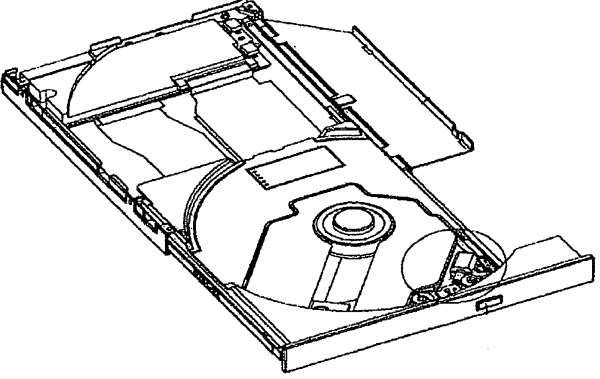
\includegraphics[width=0.38\textwidth]{images/cdrom.png}
\end{center}
\caption{Lecteur CD-ROM}
\end{wrapfigure}
Les CD-ROM ne sont plus beaucoup utilisés pour les jeux vidéos, qui dépassent maintenant souvent la capacité de stockage de ceux ci (entre 600 et 900Mo). Ils sont remplacés par des supports comme les DVD-ROM ou les Bluray. Cependant, il est intéressant d'étudier ce support de stockage pour une meilleur compréhension de l'évolution des périphériques.

Le CD-ROM a beaucoup été utilisé dans les années 90 et 2000, car le coût de fabrication de ce support est faible et ses capacité de stockage suffisantes, quitte à fournir régulièrement 4 CD-ROM dans les boites de jeu.

La vitesse de lecture de ce support est, par contre assez faible et rapidement les jeux ont utilisé ce média pour simplement installer les données sur le disque dur et servir de DRM.

\newpage
Vitesse de transfert des lecteurs CD-ROM: \cite{hardware:cdromspeed}

\begin{tabular}{|l|c|c|}
  \hline
  Vitesse du lecteur & Taux de transfert (BPS) & Latence (ms)\\
  \hline
  Single-speed (1x)&153,600&400\\
	Double-speed (2x)&307,200&300\\
	Triple-speed (3x)&460,800&200\\
	Quad-speed (4x)&614,400&150\\
	Six-speed (6x)&921,600&150\\
	Eight-speed (8x)&1,228,800&100\\
	Ten speed (10x)&1,536,000&100\\
	Twelve speed (12x)&1,843,200&100\\
	Sixteen speed (16x)&2,457,600&90\\
	Eighteen speed (18x)&2,764,800&90\\
	Twenty four speed (24x)&3,686,400&90\\
	Thirty two speed (32x)&4,915,200&85\\
	One hundred speed (100x)&15,360,000&80\\
	CAV drives (12x - 24x)&1,843,200 - 3,686,400&150-90\\
  \hline
\end{tabular}

Comme nous pouvons le constater, les temps d'accès du lecteur CD-ROM sont assez élevé. Si nous devons charger 50 petits fichiers sur un lecteur 16x, nous ajoutons inutilement 4 secondes et demi de temps de chargement. Il convient donc d'encapsuler ces 50 fichiers dans un seul, de le charger d'une traite puis de faire la séparation des fichiers en mémoire.
C'est pour cette raison que sur les CD-ROMs de jeux nous trouvons souvent que peu de fichiers, mais qui prennent une grande partie de l'espace.

\subsubsection{Lecteur DVD-ROM}
Le DVD-ROM a une vitesse 9 fois supérieure à celle d'un CD-ROM,\cite{hardware:dvdromspeed} pour une capacité allant de 4.7Go à 17.08Go (ce dernier étant très rare). Le temps d'accès aux données sur un DVD-ROM est d'environ 100ms pour les plus rapides, ce temps variant en fonction des lecteurs. Nous retrouvons donc avec les DVD-ROM le même problème qu'avec les CD-ROM : le temps d'accès au données élevé. Le taux de transfert et la quantité de données qu'il est possible de stocker sur celui ci en fait cependant un successeur de choix au CD-ROM, améliorant au passage les temps de chargement grâce à sa vitesse de lecture améliorée.

\newpage
\subsubsection{Lecteur BD-ROM}
Le BD-ROM est capable de transférer les données de 4.5Mo par seconde (x1) à 72Mo par seconde (x16)\cite{hardware:bdromspeed} et peut stocker entre 25Go et 50Go de données. Cela représente 50 fois la vitesse d'un CD-ROM. Bien que ses temps d'accès soient similaires voir plus grands que pour les DVD-ROMs, sa vitesse de transfert lui permet cependant de proposer des temps de chargement plus rapides, les données étant stockées sous forme de flux dans l'ordre d'utilisation comme pour les autres supports sous forme de disque, sa capacité de stockage permet en plus d’alléger le travail du processeur en proposant des données moins compressées.

\subsubsection{Le Disque Dur}
\begin{wrapfigure}{r}{0.4\textwidth}
\begin{center}
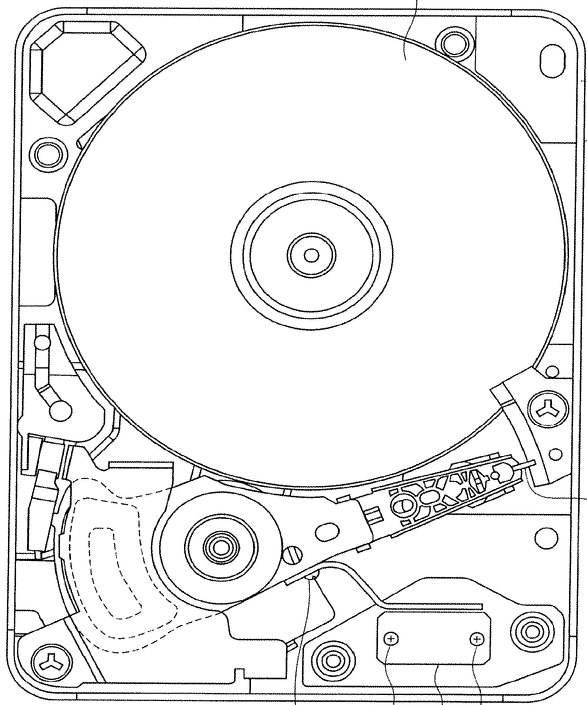
\includegraphics[width=0.38\textwidth]{images/hdd.png}
\end{center}
\caption{Disque dur}
\end{wrapfigure}
Le disque dur est le support de stockage le plus utilisé sur PC. Présent depuis les années 60 dans les ordinateurs de bureau, il a depuis continué à s'améliorer et à augmenter ses performances de lecture/écriture et ses temps d'accès. Le premier disque dur avait un temps d'accès de 600ms. Dès les années 80, ce temps a été réduit à 20ms et a continué de diminuer depuis.

Il existe 5 vitesses pour les disques durs, qui sont le nombre de rotation effectuées par le disque, par minute. Les vitesses de disque les plus répandues sont celles à 5400 tours/minute et 7200 tours/minute (respectivement 5.55ms et 4.16ms de temps d'accès moyen).\cite{hardware:hddspeed}

Les taux de transfert des disques à 7200 tours par minute en 2010 sont en moyenne de 125Mo par seconde. Comparé aux supports de stockage au format optique, le disque dur les surpasse tous. Cependant des problèmes peuvent intervenir sur les disques durs comme la corruption de données, ou la perte de vitesse à cause de la fragmentation qui peut intervenir sur certains systèmes de fichiers. Séparer les fichiers sur ce type de disque pour ne pas avoir de chargement sous forme de flux peut donc s'avérer pénalisant sur un disque fortement fragmenté.

\subsubsection{Le SSD}
Le SSD est le support de stockage qui remplace peu à peu les disques durs. Ses taux d'accès étant très faible (en dessous de 0.1ms) et sa capacité de transfert élevé (entre 100 et 550Mo par seconde)\cite{hardware:ssdspeed}, il permet d'avoir peu voire pas de chargement visible pour l'utilisateur dans les jeux vidéos. 

Les caractéristiques du SSD sont proches de celles des cassettes de jeu vidéo utilisées sur les machines avant l'ère du CD. Ce type de support permet d'avoir des jeux où les chargements sont transparents pour l'utilisateur. De plus, la fragmentation des fichiers n'a aucun effet sur un disque SSD, les données peuvent donc être séparées pour minimiser le chargement de ressources inutiles et permettre un chargement à la volée rapide.

\subsection{Multiplier les supports}
Si nous avons vu la supériorité des disques durs et SSD par rapport aux supports au format disque, nous pouvons quand même tirer partie du lecteur de disque pour améliorer encore les performances. Ainsi, nous pouvons nous servir du DVD/BD pour installer le jeu sur le disque dur, et garder une partie du disque qui servira lorsque le jeu sera lancé. Cela permettra d'accéder aux données à la fois du disque dur et sur le DVD/BD dans le jeu. C'est cette méthode qui est employée actuellement sur console, profitant du fait qu'elles soient équipées en disque dur pour réduire les temps de chargement.

%------------------------------------------------
\newpage
\section{Techniques d'optimisation}
\subsection{Généralités}
Il existe 3 façons majeures de charger les données nécessaires à un jeu en mémoire.

La première est de charger les données au démarrage du niveau ou du jeu et de les garder en mémoire tout le long du jeu. C'est la meilleure solution pour les ressources qui seront nécessaires à toutes les étapes du jeu, ou pour les ressources critiques du jeu sans lesquelles le jeu ne pourra pas tourner (cela permet de faire une vérification par la même occasion). Puisque ces données seront chargées quoi qu'il arrive, nous pouvons optimiser le temps de chargement en les chargeant dès le menu ou dès l'apparition des sponsors au début du jeu.

La deuxième façon est de charger les données nécessaires en fonction de la position du joueur et de l'orientation de la caméra. Nous pouvons charger les données aux alentours du joueur et des données plus détaillées en fonction de la direction dans laquelle le joueur regarde. Ainsi, ce sont autant de données en moins à charger au lancement du niveau ou du jeu, et cela permet d'éviter des écrans de chargement qui détériorent l’expérience de jeu de l'utilisateur.

La troisième façon est basée sur les événements : par exemple commencer à charger une zone lorsque le joueur sélectionne un objet qui lui permet de s'y téléporter, charger une séquence d'animation quand le joueur parle à un personnage qui va la déclencher, etc.

\newpage
\subsection{Stockage des données}
Pour améliorer les temps de chargement, les données sont organisées sur les disques en fonction de leurs secteurs et généralement dans un seul fichier d'archive (afin de minimiser les appels aux fonctions open et close du système d'exploitation, qui sont relativement lentes).


Ainsi notre fichier contenant les ressources reste toujours ouvert, et il ne nous reste plus qu'à lire les parties du fichier qui nous intéressent. Il convient donc d'optimiser la partie lecture pour que notre jeu charge le plus vite possible. Pour cela, il faut faire attention à la manière dont sont stockées les données, en l’occurrence leur position vis à vis des secteurs.

\begin{figure}[!h]%
\begin{center} 
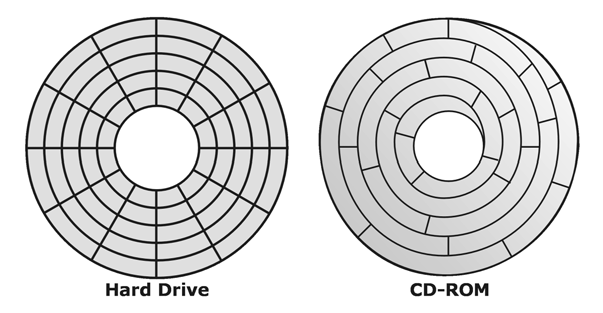
\includegraphics[width=0.60\columnwidth]{images/disk_sector.png}%
\caption{Secteurs d'un disque dur et d'un CD-ROM}%
\label{}%
\end{center}
\end{figure}

Un secteur est un fragment d'un disque qui va contenir les données stockées, un disque est composé de plusieurs secteurs mis les uns à la suite des autres. Lors d'une opération de lecture, la tête de lecture du disque ou le laser pour un disque optique va se positionner en face du secteur, et commencer à lire les données. Le temps de positionnement est le plus long, mais à chaque fois que la tête se déplacer pour parcourir un secteur, nous perdons du temps. 
Une technique pour réduire cette perte est d'aligner les fichiers sur les secteurs (ce qui entraîne une perte d'espace, si le média à un espace limité, il ne sera peut être pas possible de réaliser cette opération) \cite{industry:streaming-for-loading}.

\begin{figure}[!h]%
\begin{center} 
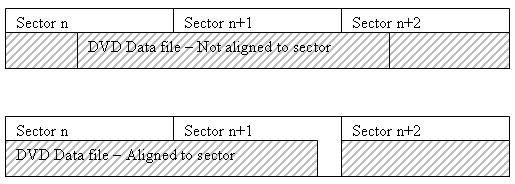
\includegraphics[width=0.60\columnwidth]{images/sector_storage.png}%
\caption{Alignement des données sur les secteurs}%
\label{}%
\end{center}
\end{figure}

\newpage
\subsection{Organisation et duplication des fichiers}
La technique la plus utilisée dans les jeux à monde ouverts disponibles sur disque optique est la technique du streaming, ou chargement par flux. Les données sont organisées sur le disque de manière à être chargées les unes à la suite des autres pour que le lecteur de disque puisse lire les données sans effectuer un nouveau tour pour se repositionner.

Si nous prenons l'exemple de Just Cause, les données du terrain sont séparées sur le disque sous forme de patch, contenant la heightmap du terrain, les textures et les données du mesh. Compte tenu du fait qu'ils avaient encore de l'espace disponible sur le disque optique, ils ont stocké les données du terrain deux fois: une fois ordonné en x vers z et une fois en z vers x. Ainsi les données peuvent être chargées sous forme de flux en fonction de la direction du joueur \cite{industry:justcause-streaming}.

Ainsi nous remarquons qu'une technique d'optimisation de chargement peut passer par la duplication des données pour s'adapter au support de stockage. A partir de ce constat nous pouvons imaginer de nombreuses possibilités pour optimiser le chargement de nos données : fichiers par flux sur le disque optique et fichiers organisés de manière séparée sur le disque dur, en chargeant les données du terrain sur le disque en flux en fonction des déplacements du joueur et celles du disque dur pour les événements aléatoires ou les chargements de ressources contenant beaucoup de données.

Une technique pour constituer les fichiers de flux est de placer des logs dans le code pour voir dans quel ordre les ressources sont chargées, ainsi il suffira de les placer dans le même ordre dans le fichier de flux.
\newpage
\subsection{Chargement en tâche de fond}
Le chargement des fichiers nécessaires pour mettre en place un jeu de type Open World peut être immédiat comme prendre plusieurs secondes pour être accompli. Ce type de jeu ne présentant normalement pas d'écran de chargement, il ne faut pas que cette tâche soit bloquante pour l'utilisateur du jeu, il faut donc prévoir un chargement en tâche de fond, qui n'altère pas l'expérience de jeu sur la machine utilisée pour jouer.

Pour effectuer ce chargement de la manière la plus fluide possible, l'équipe de Dungeon Siege l'a découpé en 3 étapes distinctes\cite{industry:dungeonsiege-streaming}: 

D'abord, les informations sur le mesh sont chargées (sans les textures et les animations), puis l'objet 3D est ajouté aux nœuds de la scène une fois chargé. Ensuite, si le mesh est dans le frustrum du joueur, la texture est chargée et appliquée à l'objet 3D. Ainsi ils économisent le chargement de la texture dans le cas ou l'objet 3D ne sera jamais rendu à l'écran. 

Notons tout de même qu'en cas de déplacement brusque ou de nombreux objets à afficher, il se peut que le joueur aperçoive un court instant des objets 3D sans texture. Pour améliorer cela, nous pouvons charger les textures en fonction de l'espace mémoire disponible pour les objets proches du joueur, qu'ils soient dans le frustrum ou non.

Ce découpage permet d'annuler le chargement en cours de route si le joueur décide de changer de direction ou passe trop vite pour que l'objet soit dans son champ de vision.

Le chargement en tâche de fond prend aussi des ressources processeur, utilisée par le jeu en tâche principale et ce à cause notamment de la compression des fichiers (voir section Optimisation par compression). Il convient donc de limiter cet usage pour laisser au jeu le plus possible de capacité de calcul pour que le chargement ne fasse pas chuter les taux de rafraîchissement.

\newpage
\subsection{Définir des zones}
Pour permettre un jeu fluide et éviter les écrans de chargements, il convient d'anticiper les déplacements du joueur et de connaitre les zones qu'il peut potentiellement visiter. Ainsi, il est utile de connaître la zone dans laquelle est placé le joueur ainsi que les zones qui l'entourent. Lorsqu'un joueur visitera une zone, les zones d'à côté seront chargées en tâche de fond et celles qui sont éloignées seront déchargées ou gardées uniquement sous forme simplifiée.

\begin{wrapfigure}{l}{0.5\textwidth}
\begin{center}
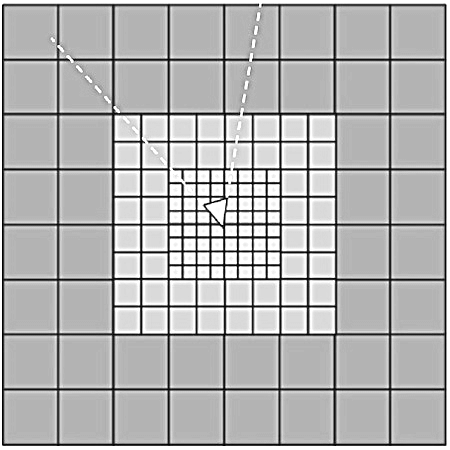
\includegraphics[width=0.45\textwidth]{images/patch-system-three.png}
\end{center}
\caption{Système de patch}
\end{wrapfigure}

La figure ci contre représente un système de patch sous forme d'arbre avec plusieurs niveaux de détail. Au centre, les patch sont détaillés et découpés en petites zones et sont chargées avec tout leur contenu en mémoire. Les cellules moyennes qui sont plus éloignées du joueur, sont elles chargées de manière incomplète (seul les données importantes au rendu à moyenne distance: données terrain, textures, habitations, arbres, etc.). Les patch plus gros sont eux chargés grossièrement, pour avoir un rendu simpliste nécessitant peu de ressources. Ainsi en fonction du déplacement du joueur, les zones autour de lui vont changer en suivant la même direction pour passer en mode détaillé, moyen ou léger. Un problème peut survenir dans le cas où le joueur se déplace de manière rapide. Dans ce cas, seul les zones contenues dans le frustrum pourront passer en détaillé, tandis que les celles derrière le véhicule et sur les côtés pourront passer plus rapidement en mode léger.

Un second problème se pose dans le cas ou un déplacement instantané peut survenir (téléportation). Pour résoudre en partie ce problème, il convient de trouver les zones dans lesquelles le joueur va pouvoir se téléporter et de les charger en mode moyen à l'avance si l'espace mémoire le permet, même si elles ne sont pas voisines. Ainsi le joueur pourra être téléporté et la zone finira de charger du mode moyen au mode détaillé en cours de route. Ce processus peut intervenir à proximité d'un portail de téléportation, ou lorsque le joueur est dans son inventaire et possède des objets qui lui permettent de se téléporter.

\subsection{Prioriser les chargements}
Une technique pour rendre les chargements le plus discret possible serait de définir un ordre de priorité pour les ressources et objets à afficher. 

Par exemple, nous pouvons retarder le chargement et l'apparition d'un objet qui n'a qu'une utilité esthétique dans notre jeu ou notre scène. Les objets à charger en premier lieux sont ceux avec lequel le joueur peut entrer en interaction (levier, bouton sur lequel le joueur doit appuyer, porte, etc.) pour qu'il puisse continuer à avancer dans avoir à attendre que les objets apparaissent ou qu'il ne se retrouve pas bloqué sans comprendre ce qu'il se passe. Les murs et le terrain, même s'ils ne sont pas des objets interactifs doivent être chargés également car sans eux le joueur se déplacerait dans le vide et n'aurait aucun moyen de se repérer dans l'espace.

Les objets à charger en suite sont les NPC, ou personnages non joueur: un animal dans le décors que le joueur peut tuer pour récolter des ressources, ou un personnage donneur de quête par exemple. Ceux ci ne sont pas critiques pour l'avancée du joueur et souvent nécessitent un certain nombre de ressources (modélisation, sons et animations) ainsi il convient de les charger en second lieux. 

Viennent en dernier lieux les objets de décoration, la végétation, et les sons. Cela ne pose pas de problème de permettre au joueur d'avancer avant d'entendre ses bruits de pas par exemple. Avoir différentes textures de fleur pour un sol en plein air n'est pas important pour le joueur, tout comme des tuyaux qui viendraient joncher un couloir. Les charger en dernier permet d'avoir un affichage rapide des niveaux et de réduire au maximum les temps d'attente du joueur.

\newpage
\subsection{Perception du chargement}
Si les chargements sont inévitables, il convient de définir clairement le moment où ils vont intervenir. Les joueurs ont tendance à accepter d'avantage les chargements à des moments particulier du jeu vidéo. Par exemple, il faut que le jeu expose un rendu rapidement à l'écran après son lancement, et que le menu soit affiché peu après, pour avoir l'impression d'un chargement moins lourd. 

Nous avons déjà pu expérimenter des jeux qui mettent de nombreuses secondes à démarrer entre le lancement du binaire et l'affichage de la première image. Ce temps semblera sensiblement moins long à l'aide d'un splash screen, pour confirmer que le jeu est en train de charger et faire patienter le joueur. Si le splash screen propose une animation, le temps de chargement sera encore moins long.

Une astuce trouvée par de nombreux jeux est de proposer une petite animation lors du chargement du jeu, animation contrôlable en partie par le joueur. Ainsi il peut passer le temps en réalisant un mini jeu ou en contrôlant un petit personnage. Les temps de chargements semblent alors beaucoup moins long.

Historiquement, les joueurs sont habitués à devoir attendre entre le menu et le chargement du niveau ou du jeu, il est donc conseillé de placer le maximum de chargement à ce moment là. Par exemple dans Donkey Kong Country Tropical Freeze, tous les chargements sont effectués entre le menu et la carte du monde. Une fois le niveau lancé, un chargement très court intervient pour charger le peu d'assets manquants et générer le niveau. Si la totalité du niveau était chargé au moment de sa sélection sur la carte du monde, ces mêmes chargements deviendraient un défaut notoire.

\newpage
\subsection{Préparer des billboards}
Les billboards sont les textures qui remplacent les objets 3D au loin dans les jeux, pas exemple les arbres. Ils font toujours face à la caméra du joueur et sont généralement rafraîchies que lorsque le joueur se déplace d'une certaine distance par rapport à sa position de base lorsque le billboard a été calculé la première fois. 

\begin{figure}[!h]%
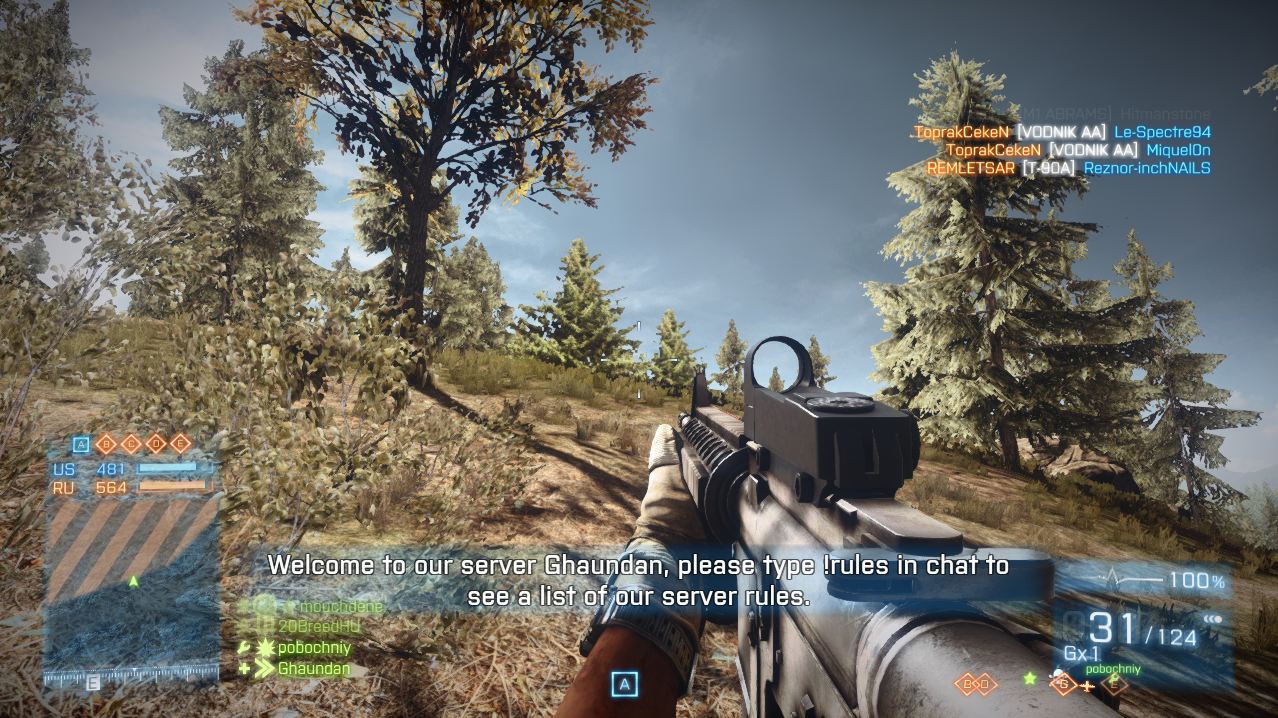
\includegraphics[width=\columnwidth]{images/bf3_billboards.png}%
\caption{Billboards dans Battlefield 3 (arbres au loin)}%
\label{}%
\end{figure}

Nous pouvons nous inspirer de cette technique pour améliorer les temps de chargement, en préparant au préalable des billboards pour certains objets 3D non prioritaires qui seront alors chargés en premier lieu sous la forme de billboards. Si nous prenons l'exemple d'un joueur qui entre dans une maison et se dirige à proximité de la cuisine, nous pouvons lui afficher les tasses et couverts qui sont posés sur la table sous la forme d'un billboard, et si le joueur s'attarde dans cette même cuisine ou si le CPU le permet et qu'il n'y a pas d'autres objets plus prioritaires à charger dans la queue, nous chargeons le vrai objet 3D.


\newpage
\subsection{Utiliser du LOD}
Le LOD signifie Level of Detail et est une technique qui permet d'améliorer les performances graphiques en fonction de la distance des objets. Ainsi les objets qui sont situés le plus loin sont affichés de manière rudimentaire, avec des textures légères et très peu de polygones et d'animation.

Nous pouvons nous servir de cette technique pour améliorer les chargements, en ne chargeant au départ que les ressources qui sont en format léger, et charger les versions complètes des objets une fois dans le jeu si l'utilisation du processeur le permet. Cette technique ressemble à celle des zones décrit plus haut, qui consiste à charger des versions légères en fonction de la distance des objets par rapport aux joueurs.

Cependant ici nous chargeons même les zones à proximité du joueur en mode léger, dès le départ afin de réduire le plus possible le premier écran de chargement. Ceci est une technique acceptable pour certains types de jeu où le décor ne joue pas un rôle important. Cependant si nous souhaitons mettre l'accent sur les graphismes ou si nous ne voulons pas que le joueur ressente ce chargement qui peut être plus ou moins long et plus ou moins dérangeant selon les sensibilités, il faudra éliminer cette possibilité.

%------------------------------------------------
\newpage
\section{Optimisation par compression}
\subsection{Généralités}
La compression de données regroupe un ensemble de techniques permettant de réduire considérablement le volume de données avec ou sans perte d'information. On utilise généralement des algorithmes qui permettent de compresser les données. Si l'algorithme utilisé est sans perte, la totalité des données compressées est récupérée lors de la décompression tandis que si l'algorithme est avec perte, seule une partie des données originales est récupérée (on essaie alors de garder les informations pertinentes). La perte reste minime en fonction des algorithmes utilisés ce qui rend la reconstruction de l'information raisonnable et satisfaisante. 

\begin{figure}[!h]%
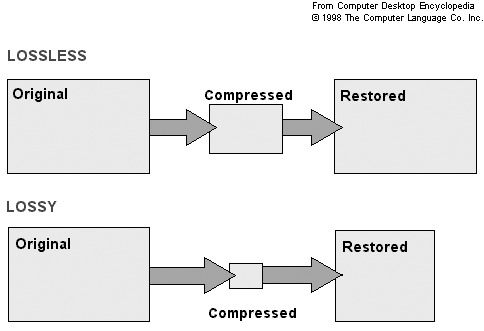
\includegraphics[width=\columnwidth]{images/data_compression.png}%
\caption{Compression des données avec et sans perte}%
\label{}%
\end{figure}

Un fichier compressé prend moins de place sur un support de stockage qu'un fichier non compressé, cela permet de réduire le temps de passage d'un fichier du support de stockage à la mémoire de l'ordinateur ou de la carte graphique. Autrement dit le volume de la donnée compressée est plus petit, de même le temps des transferts est réduit. Puisque la taille des données contenues dans les jeux est parfois très grande, il serait impensable de les stocker sur le support de stockage sans les compresser au préalable. De plus en plus, la compression devient quasiment indispensable pour stocker la totalité d'un jeu. En effet, même si la capacité et les performances des différents composants des ordinateurs ou des consoles évoluent d'année en année, le volume des données est tellement grand que nos machines ne parviennent pas toujours à gérer une quantité aussi grande d'information.

Dans les jeux vidéo de nombreux éléments sont utilisés et doivent être stockés (images, sons, objets 3D, etc.). De ne jours, la totalité des données d'un jeu peut être contenue sur un disque et il s'agit très souvent de données compressées qui doivent être décompressées lors de leur chargement en cours de jeu.

Étant donnée la diversité des éléments qui composent un jeu, plusieurs techniques spécifiques sont parfois nécessaires pour compresser et décompresser tel ou tel type de fichier. Ainsi les images, les vidéos et les sons ne seront pas forcément traités de la même manière. Ces éléments sont souvent très volumineux et le but est de parvenir à les compresser au maximum pour atteindre une vitesse de transfert satisfaisante tout en conservant un niveau de qualité le plus élevé possible. 

Les données des images et des vidéos sont mesurés par un nombre d'unité binaire (bits), c'est pourquoi on parle de vitesse de transfert de bits (bit rate) comme étant le paramètre principal lors de la compression de données. 

\newpage
\subsection{Compression des images}
Les images sont très utilisées et en grande quantité dans les jeux vidéo. C'est pourquoi la compression joue un rôle très important. Ils existent plusieurs algorithmes de compression qui permettent de comprimer les images. Bien entendu, certaines méthodes seront plus adaptées pour un type d'image particulier que pour un autre. 

Voici les différents types d'images et leurs caractéristiques : 

\begin{tabular}{|p{0.1\columnwidth}|p{0.25\columnwidth}|p{0.55\columnwidth}|}
  \hline
  Format & Nom & Caractéristique\\\hline\hline
  BMP&Windows bitmap&Format non compressé\\\hline
	TIFF&Tagged Image File Format&Sans perte\\\hline
	PNG&Portable Network Graphics&Sans perte, amélioration du format GIF. Basé sur l'algorithme de compression Deflate\\\hline
	JPEG&Joint Photographic Experts Group&Avec perte, taux de compression élevé\\\hline
	JPEG 2000&Joint Photographic Experts Group 2000&Avec perte, une amélioration du format JPEG\\\hline
\end{tabular}

Quelques remarques concernant ces différents formats d'image : 

\begin{itemize}
  \item Le format JPEG a un taux de compression élevé, réduisant ainsi la qualité de l'image. Il est idéal pour les grandes images et les photos.
	\item Le format PNG est un algorithme de compression sans perte. Il est très efficace pour des images contenant peu de couleurs différentes ou possédant des grandes zones contenant une couleur unie.
	\item Il est préférable d'utiliser le format PNG pour des images contenant du texte.
	\item Le format JPEG 2000 a un taux de compression supérieur à celui du format JPEG.
\end{itemize}

Voici les résultats récupérés dans le document "Comparison of different image compression formats"\cite{compression:images-compression-formats} présentant les tests de Paula Aguilera concernant les différentes type de compressions d'image :

\subsubsection{Compression sans perte}
Pour une image de 24 bit de profondeur de couleur pesant 696KB dans un format BMP contenant de nombreuses zones de couleur homogène.

\begin{center}
\centering
	\begin{tabular}{|l|c|c|}
		\hline
		Format & Poids (en KB)& Taux de compression\\
		\hline
		BMP&696&1:1\\
		TIFF-LZW&378&2:1\\
		PNG&258&2.7:1\\
		JPEG&43.3&16:1\\
		\hline
	\end{tabular}
\end {center}

Pour une image en niveau de gris pesant 257KB dans un format BMP contenant beaucoup de détails.
\begin{center}
\centering
	\begin{tabular}{|l|c|c|}
		\hline
		Format & Poids (en KB)& Taux de compression\\
		\hline
		BMP&257&1:1\\
		TIFF-LZW&251&1:1\\
		PNG&173&1.5:1\\
		JPEG&79&3.2:1\\
		\hline
	\end{tabular}
\end{center}

\subsubsection{Compression avec perte}

Pour une image de 24 bit de profondeur de couleur pesant 768KB dans un format BMP contenant des couleurs vives et des textures. Pour une compression au format JPEG, on peut choisir le degré de qualité que l'on souhaite conserver lors de la compression. Il s'agit d'un nombre entre 1 et 100, plus le chiffre est grand plus le taux de compression sera faible et donc plus la qualité d'image sera élevée. Voici les résultats des tests avec une compression au format JPEG avec des niveaux définis à 100, 50, 10 et 1.

\begin{center}
	\begin{tabular}{|l|c|c|}
		\hline
		Format & Poids (en KB)& Taux de compression\\
		\hline
		BMP&768&1:1\\
		TIFF&768&1:1\\
		PNG&768&1:1\\
		JPEG - 100&334&2.3:1\\
		JPEG - 50&49.5&15.5:1\\
		JPEG - 10&16.3&47:1\\
		JPEG - 1&6.3&121:1\\
		\hline
	\end{tabular}
\end{center}

D'après ces tests, les compressions en format PNG et TIFF ne sont pas efficaces à cause des couleurs vives et des textures. 

De manière générale, lors d'une compression le format PNG est un très bon choix car le taux de compression est raisonnable avec une qualité d'image satisfaisante, tandis que le format JPEG donnera un taux de compression élevé mais une qualité d'image moins intéressante. Même si le poids des images JPEG est plus faible que celles en PNG, leur qualité est appauvrie par la compression. 

Il faut ensuite s'intéresser au temps de chargement nécessaire pour décompresser le fichier en mémoire pour pouvoir l'utiliser et cette étape du chargement sollicite le processeur.

\subsection{Compression des meshes}
Les jeux vidéo utilisent généralement des meshes (maillages) représentant toutes les formes possibles (personnages, bâtiment, véhicules, objets, etc.). Dans le domaine des jeux vidéo, on préfère avoir des maillages composés uniquement de triangles pour leur simplicité. Le nombre de polygones que les machines peuvent afficher est limité, c'est pourquoi on utilise les maillages. Ces formes sont plus ou moins complexes et doivent souvent être compressées pour des questions de volume et de transfert. Pour des jeux en 3D, une carte graphique peut afficher des milliers de polygones (en 2005, une carte graphique pouvait afficher 180 millions de triangles par secondes)\cite{compression:meshes}.

\begin{figure}[!h]%
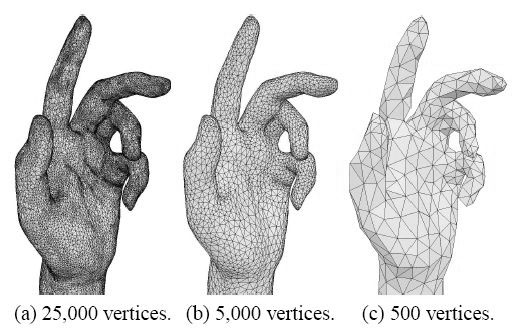
\includegraphics[width=\columnwidth]{images/meshes.jpg}%
\caption{Différents maillage de la surface d'une même forme}%
\label{}%
\end{figure}

Une forme contenant de nombreux triangles sera plus complexe et donc plus détaillé qu'une forme simple qui en contient moins.

Plus le nombre de polygones que l'on souhaite afficher à l'écran est élevé, plus les capacités de la machine seront sollicitées. Dans les jeux 3D à monde ouvert, il faut charger et afficher les éléments de l'environnement les plus proches du joueur mais aussi parfois les plus éloignés (paysages lointains par exemple). Le but est alors de réussir à charger ces différents objets le plus rapidement possible pour que le jeu soit fluide (le joueur préfère ne pas voir les objets apparaître devant son personnage). La vitesse de chargement des meshes dépend de leur taille, du nombre de polygones dont ils sont composés et des ressources de la machine. En effet il faudra plus de temps pour charger un objet très détaillé (définit par de nombreux polygones) qu'un objet simple. Une astuce consiste à réaliser des meshes complexes pour les éléments qui seront affichés près de la caméra, tandis que pour des éléments qui seront toujours éloigné du personnage tel que les montagnes ou les nuages, il s'agira plutôt de meshes simplifiés. Grâce à cette méthode, la vitesse de chargement de l'environnement est relativement plus rapide.

La compression des meshes permet aussi d'obtenir des fichiers moins volumineux. On distingue toujours la compression avec ou sans perte. La première insiste sur le fait que certains détails seront supprimés avant la compression, il s'agit en général d'éléments jugés non perceptibles par l’œil humain lors de la visualisation. 

\newpage
\subsection{Compression des vidéos}
Dans la plupart des jeux, des cinématiques sont utilisées pour mettre en scène l'histoire du jeu. Elles peuvent être réalisées directement avec le moteur du jeu à l'aide d'animations. Souvent, il s'agit plutôt de vidéos en images de synthèses. On les retrouve généralement au démarrage du jeu avant l'écran titre mais aussi avant chaque mission pour présenter la situation. Ces vidéos doivent donc être chargée puis diffusée. Tout comme pour le chargement des objets 3D et les images on peut penser qu'il faut un certain temps à la machine pour effectuer cette action. 

Les vidéos prennent beaucoup de place sur le support, ceci est dû à la quantité d'informations qu'elles contiennent. Même si les machines d'aujourd'hui sont de plus en plus performantes il est encore difficile de penser que l'on peut stocker toutes les données d'un jeu sans les compresser. Dans ce cas, il faudrait des dizaines de gigaoctet (voire des centaines) d'espace mémoire pour stocker ces données sur le support de stockage. De plus, le chargement d'une telle quantité d'informations risquerait de prendre énormément de temps, ce qui ruinerait totalement l'expérience de jeu. On se rappelle alors des premiers jeux de la Sony Playstation qui demandaient des temps de chargement élevés pour parvenir à récupérer les données nécessaires pour la scène de jeu en cours. Ce problème s'appliquait aussi aux vidéos qui devaient être chargées en mémoire, lues, puis déchargés pour laisser place au chargement des autres données.

Il est donc plus judicieux de réussir à réduire la taille des données et ce par la compression mais aussi la décompression lors du chargement. En ce qui concerne les vidéos, on parlera aussi de méthodes de codage vidéo.

Le but est donc de choisir le meilleur format de compression. Voici un tableau montrant le standard de compression vidéo, dont le format CIF est la base d'une hiérarchie de format.

\begin{center}
	\begin{tabular}{|l|p{0.25\columnwidth}|c|l|}
		\hline
		Format & Résolution Luminance (H x V) & Bits par image & Application\\
		\hline
		Sub-QCIF&128 x 96&147 456&Vidéo mobile\\
		Quarter CIF&176 x 44&304 128&Vidéo conférence\\
		CIF&352 x 288&147 456&Monitoring vidéo\\
		4CIF&704 x 576&4 866 048&TV, DVD\\
		720i50&1280 x 720&11 059 200&HD TV\\
		1080i50&1920 x 1080&24 883 200&HD DVD\\
		\hline
	\end{tabular}
\end{center}

La compression d'une vidéo consiste en fait à encoder les données qu'elle contient pour éliminer les parties redondantes ou inutiles qui ne sont pas nécessaires à la récupération de la vidéo d'origine lors de la décompression. L'encodage est définit par quatre modules : la prédiction, la transformation, la quantification et le codage entropique. Voici les étapes effectuées lors de l'encodage de la vidéo \cite{compression:video} :

\begin{itemize}
  \item On fournit à l'encodeur la vidéo d'origine.
	\item La prédiction exploite la redondance entre les trames voisines, ce qui lui permet de construire une prédiction des trames suivantes.
	\item Le module de transformation convertit le résultat de la prédictions : transformation de la trame en coefficients.
	\item Les coefficients sont quantifiés en série de coefficients significatifs qui représentent alors de manière plus compacte la trame résiduelle d'entrée.
	\item Les valeurs quantifiées sont finalement compressées par le codage entropique.
\end{itemize}

En ce qui concerne le rôle du décodeur, il reconstruit la vidéo à partir de la séquence obtenue lors de l'encodage.

\subsubsection{Prédiction}
Dans une vidéo, on constate que deux images successives sont relativement identiques. En effet, si la vidéo présente l'animation d'un personnage dans un décor particulier, on peut observer que certains éléments restent inchangés d'une image à l'autre, seul le personnage ou une partie de son corps bouge. Cela permet de définir quelles informations sont redondantes ou non. Ainsi, le module de prédiction obtient un résidu définissant la différence entre les différentes trames.

\newpage
\subsubsection{Transformation}
La transformation permet de compacter la trame obtenue suite à la prédiction. Il existe plusieurs transformées permettant d'effectuer cette tâche, par exemple la Transformée Cosinus Discrète (DCT) qui se base sur des blocs et la Transformée Ondelette Discrète (DWT) basée sur une image entière. Il semblerait que la DWT soit plus performantes que la DCT mais elle nécessite trop de mémoire.

\subsubsection{Quantification}
La transformation permet d'obtenir des coefficients qui ont des valeurs parfois très proches. La quantification est alors utilisée pour garder un petit nombre de coefficients significatif. Il s'agit alors de la représentation compacte de la trame résiduelle.

\subsubsection{Codage entropique}
Les coefficients quantifiés doivent encore être codées pour les compresser encore plus avec le stockage et la transmission. Le but du codage entropique est d'assigner des codes courts aux symboles les plus récurrents. Le codage Huffman modifié et le codage arithmétique sont deux types de codage entropique.

\begin{figure}[!h]%
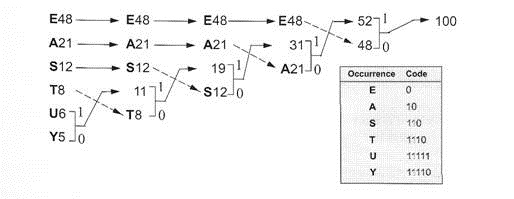
\includegraphics[width=\textwidth]{images/codage_huffman.jpg}%
\caption{Codage Huffman}%
\label{}%
\end{figure}

Une fois ces étapes réalisées, le stockage peut être effectué. Lorsque la vidéo est demandée par le jeu, le programme charge la vidéo, il doit alors décoder la séquence obtenue lors de la compression. Le temps de décompression est variable en fonction de la taille des données à traiter. 

Les organisations internationales de standardisation l'UIT-T et l'ISO/IEC ont développés des standards de compression vidéo tel que le MPEG-4, format utilisé par les jeux vidéo. Une amélioration de ce format, le MPEG-4 H.264 permet lors de la compression d'obtenir un codec plus performant.

Voici les différentes versions du format MPEG :

\begin{center}
	\begin{tabular}{|p{0.2\columnwidth}|p{0.15\columnwidth}|p{0.55\columnwidth}|}
		\hline
		Format & Période de développement & Application\\
		\hline
		MPEG-1&1988-1996&Lecteur VHS, stockage de sons et d'image pour CD interactifs\\
		MPEG-2&1990-2000&Diffusion télévisuelle, réseaux et support DVD\\
		MPEG-4&1993-2003&Consoles de jeux vidéo, réseaux sans fil, téléphone cellulaire, satellite\\
		H.26X et H.264 AVC (Advanced Video Coding)&1999-2003&Application de communication à très faible débit de transmission (téléphonie, jeux en ligne, réseaux sans fil)\\
		\hline
	\end{tabular}
\end{center}

Le MPEG-4 est un format standard de compression vidéo souvent utilisé dans les jeux vidéo. Les performances du codec au niveau de la compression et de la vitesse de transmission en font un choix efficace. 

On peut supposer que lorsqu'une vidéo est lue pendant le jeu, un programme permet de charger en fond les données de la séquence de jeu qui suit. Cette technique peut être efficace pour optimiser le temps de chargement. Ainsi le joueur pourra jouer directement une fois la vidéo terminée.

\newpage
\subsection{Compression des sons}

Il existe de nombreux formats de compression audio. Comme pour toutes compressions de données, elle peuvent être avec ou sans perte. Dans tous les cas, le but est de choisir le format dans lequel le taux de compression et la qualité sont satisfaisantes, mais on souhaite aussi que la vitesse de transmission soit la plus rapide possible.

Dans les jeux vidéo, il existe des sons pour presque tous les éléments : décors, objets, personnages, actions, environnement, etc. Le jeu doit souvent lancer plusieurs sons simultanément pour cet différents éléments. C'est pourquoi il faut que la machine puisse charger plusieurs sons à la fois et ce rapidement. Une technique consisterait à charger en mémoire les sons les plus utilisés à un moment donné du jeu, pour pouvoir les jouer immédiatement lorsqu'ils sont appelés, mais cette méthode nécessite du matériel performant capable de stocker une grande quantité d'informations en mémoire.

Il est donc préférable de trouver le format de compression idéal pour que celle-ci soit la plus efficace, avec le moins de perte possible et avec décompression qui se fasse rapidement.

Voici un tableau réunissant quelques formats de compression audio :

\begin{center}
	\begin{tabular}{|p{0.25\columnwidth}|p{0.25\columnwidth}|p{0.2\columnwidth}|p{0.15\columnwidth}|}
		\hline
		Format & Algorithme & Vitesse de transfert (kbits/s) & Latence (ms)\\
		\hline
		ALAC & Sans perte & - & -\\
		FLAC & Sans perte & - & 4.3 - 92\\
		Monkey's audio & Sans perte & - & -\\
		RealAudio & Sans perte & - & - \\
		True Audio & Sans perte & - & - \\
		WavPack & Sans perte & - & - \\
		Windows Media Audio & Sans perte & - & >100\\
		\hline
		AAC & MDCT-Hybrid, Subband & 8 - 529 & 20 - 405\\
		ATRAC1 & MDCT-Hybrid, Subband & 292 & >100\\
		ATRAC3 & MDCT-Hybrid, Subband & 66 - 132 & >100\\
		ATRAC3plus & MDCT-Hybrid, Subband & 48 - 352 & >100\\
		MP3 & MDCT-Hybrid, Subband & 8 - 320 & >100\\
		Musepack & Subband & 3 - 1300 & - \\
		OGG Vorbis & MDCT & 8 - 768 & >100\\
		Windows Media Audio & MDCT & 8 - 768 & >100\\
		\hline
	\end{tabular}
\end{center}

Le format OGG est le plus souvent utilisé par les jeux vidéo du fait qu'il s'agisse d'un format ouvert et libre. Le MP3 est aussi un format très utilisé. On constate d'après le tableau que la vitesse de transfert est plus élevé avec le format OGG. Ce format est une compression obtenue à partir de différents algorithmes générant un fichier son qui, lorsqu'il est décompressé par le décodeur, reste fidèle au son d'origine pour l'oreille humaine. En effet, en utilisant ce format audio, notre oreille parvient difficilement à percevoir les différences entre le fichier compressé et le fichier original malgré la perte d'informations générée par la compression.

\subsection{Tableau des formats de compression multimédia}

\begin{center}
	\begin{tabular}{|p{0.1\columnwidth}|p{0.2\columnwidth}|p{0.6\columnwidth}|}
		\hline
		Type & Norme & Formats\\
		\hline
		Vidéo & ISO/CEI & MJPEG, Motion JPE 2000, MPEG-1, MPEG-2, MPEG-4 ASP, MPEG-4/AVC, HEVC\\
		\cline {2-3}
			& UIT-T & H.120, H.261, H.262, H.263, H.264, HEVC\\
		\cline {2-3}
			& On2 & VP3, VP5, VP6, VP7, VP8, VP9\\
		\cline {2-3}
			& Autres & AMV, AVS, Bink, Cinepak, Dirac, Indeo, jpg.rem, Pixlet, RealVideo, rem, RTVideo, SheerVideo, SmackerSmacker, Snow, Sorenson, Theora, VC-1, WMV\\
		\hline
		Audio & ISO/CEI & MPEG-1 Layer III (MP3), MPEG-1 Layer II, MPEG-1 Layer I, Advanced Audio Coding, AAC, AAC+, eAAC+, SBR, Parametric Stereo \\
		\cline {2-3}
			& UIT-T & G.711, G.719, G.722, G.722.1, G.722.2, G.723, G.723.1, G.726, G.728, G.729, G.729.1, G.729a\\
		\cline {2-3}
			& Autres & AC3, AMR, Apple Lossless, ATRAC, CELT, FLAC, iLBC, Monkey's Audio, u-law, Musepack, Nellymoser, OptimFROG, Opus, RealAudio, RTAudio, SHN, Siren, Speex, TAK, Vorbis, WavPack, WMA\\
		\hline
		Image & ISO/CEI/UIT-T & JPEG, JPEG 2000, JPEG-LS, JBIG, JBIG2, PNG, WBMP\\
		\cline {2-3}
			& Autres & BMP, GIF, ICER, ILBM, PCX, PGF, TGA, TIFF, JPEG XR/HD Photo, EMF/WMF, WebP\\			
		\hline
	\end{tabular} 
\end{center}

\newpage
\subsection{Compression des textures}
\subsubsection{Généralités}
Les jeux sont de plus en pus réalistes que ce soit au niveau sonore ou au niveau graphique. Pour les jeux à monde ouvert, de nombreux objets sont affichés à l'écran, ils peuvent être plus ou moins détaillés et donc avoir une qualité particulière en fonction de leur type et surtout de leur importance pour l'expérience de jeu proposé par les développeurs. 

La plupart des objets utilisés dans les jeux vidéo possèdent une texture : c'est une image en 2D qui est appliquée sur une surface ou un volume permettant de l'habiller. Il s'agit d'une sorte de papier peint qui peut être déformé en fonction de la forme sur laquelle on l'applique, ces textures sont alors plus ou moins complexes.

\begin{figure}[!h]%
\begin{center}
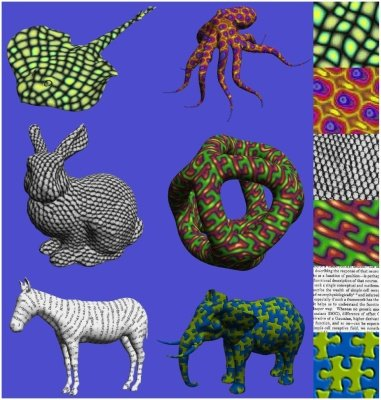
\includegraphics[width=0.8\columnwidth]{images/texture.jpg}%
\caption{Exemples de textures appliquées sur des objets 3D}%
\label{}%
\end{center}
\end{figure}

Puisque ces textures sont de plus en plus détaillées et de bonne qualité, le fichier peut être très volumineux. Lorsque plusieurs objets sont affichés à l'écran, il faut charger en mémoire leur texture, ce qui demande énormément de ressources. Il est donc important de soulager le travail du processeur et de faire en sorte que le chargement de tels éléments se fassent le plus rapidement possible pour pouvoir libérer de l'espace mémoire. Ainsi, il est conseillé de compresser les textures. Bien entendu il existe plusieurs techniques plus ou moins efficaces.

Nous allons présenter quelques algorithmes de compression de texture pouvant être utilisé avec Direct3D (une bibliothèque logicielle de DirectX de Microsoft, moteur de rendu graphique en 3D sur les systèmes d'exploitation Windows) et OpenGL. nous nous intéresserons donc aux formats de compression DXT (S3TC), 3Dc et A8L8. Chacun de ces formats sont plus ou moins utilisés et possèdent leurs propres forces et faiblesses.

\newpage
\subsubsection{Le format de compression DXT}
Il s'agit d'un standard de Direct3D et il existe plusieurs versions de cette méthode : DXT1, DXT2, DXT3, DXT4, DXT5 ; chacune étant utilisée pour un type d'image spécifique. La méthode générale consiste à représenter des blocs de 4x4 pixels à l'aide de bits. Un pixel sera défini par 4 bits si on utilise DXT1 (pas obligatoirement de bit utilisé pour l'alpha, si l'alpha est utilisé, on utilisera seulement 1 bit). Un pixel sera représenté par 8 bits pour DXT2, dont les 4 bits supplémentaires définiront l'alpha. Avec cet algorithme de compression avec perte, on obtient des blocs de 4x4 pixels pouvant aller de 64 à 128 bits, permettant d'avoir un taux de compression variant de 4:1 à 6:1. En fonction de la version que l'on utilise, on peut obtenir des images moins lourdes en mémoire au détriment de la qualité. En effet, les images seront définies par plus ou moins de bits, donc plus ou moins d'information pour chaque composante de couleur et d'alpha.

\begin{figure}[!h]%
\begin{center}
	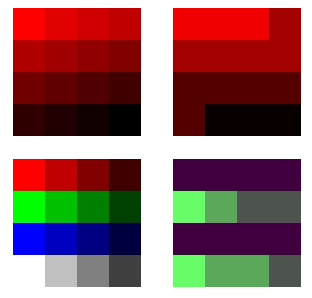
\includegraphics[width=0.5\columnwidth]{images/texture_dxt.png}%
	\caption{Résultats de la compression DXT1}%
	\label{}%
\end{center}
\end{figure}

On constate sur l'image ci-dessus que le résultat de la compression n'est pas très fidèle à l'image d'origine : il y a moins de variation dans les couleurs. Ceci s'explique par le fait qu'on utilise moins de bits pour représenter chaque composant et donc qu'on stocke moins d'information. Il est donc parfois préférable d'opter pour une version plus récente de cet algorithme pour avoir une qualité supérieure en ayant un taux de compression plus faible mais restant satisfaisant.

Cette méthode n'est pas utilisable pour tous les types d'image. En effet, il est déconseillé de s'en servir pour compresser des images dessinées à la main (effet cartoon) ou pour des normal map. Ceci est dû au fait que ce type d'image souhaitant simuler un effet de relief contiennent des variations de couleur souvent très brutales, or la compression au format DXT permet plutôt de gérer des images ayant des variations plus faibles entre les pixels voisins.


\begin{figure}[!h]%
	\begin{center}
	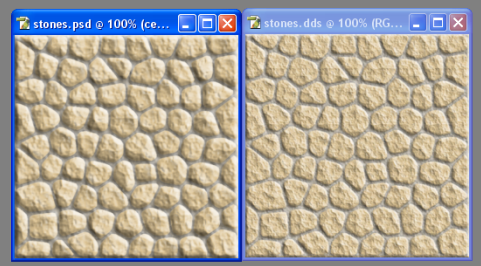
\includegraphics[width=0.60\columnwidth]{images/dxt_compression_1.png}%
	\caption{Compression DXT efficace}%
	\label{}%
	\end{center}
\end{figure}

\begin{figure}[!h]%
	\begin{center}
	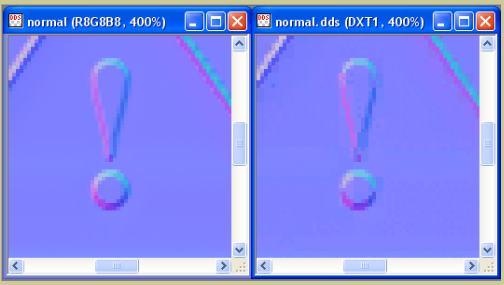
\includegraphics[width=0.60\columnwidth]{images/dxt_compression_2.png}%
	\caption{Compression DXT peu efficace : normal map}%
	\label{}%
	\end{center}
\end{figure}

Cependant il existe tout de même des astuces pour pouvoir utiliser cette méthode de compression pour compresser les normal map. Ces images contiennent comme leur nom l'indique une normale qui peut être extraite. Ce vecteur normal n'est pas obligatoirement de longueur 1, c'est ce qui provoque un rendu peu convenable lors de la compression des normal map avec le format de compression DXT. Le but est alors de renormaliser cette normale à 1. Ainsi le rendu sera meilleur, mais la qualité de celui-ci ne sera pas parfaite. Une deuxième astuce basée sur une technique utilisée dans Doom 3 permet d'obtenir un meilleur rendu. Cette technique exploite deux particularité du format de compression DXT5 :

\begin{itemize}
	\item Le canal alpha est compressé indépendamment des canaux rouge, vert et bleu. Donc celui-ci n'est pas trop altéré par la compression.
	\item Les canaux RGB sont codés sur 16 bits (5 bits pour le rouge, 6 bits pour le vert, 5 bits pour le bleu). Ainsi le vert est beaucoup plus précis.
\end{itemize}

Le but est alors de se servir de ces deux particularités pour réordonner les données liées aux canaux RGBA. La formule mathématique suivante : z = sqrt(1 - x*x + y*y); montre qu'il est possible d'obtenir z à l'aide de x et y. Ainsi les normal map ont seulement besoin de stocker les valeurs des coordonnées x et y. Chaque texel contient le triplet RGB (R représente la coordonnée x, vert le y et bleu le z). Ainsi, on utilise la première particularité pour stocker R dans A. Et on utilise la deuxième pour le calcul de z à l'aide de y. C'est la fonctionnalité appelée le ``swizzling'' qui permet de réarranger les différents composantes d'un vecteur. Cette fonctionnalité est disponible dans les langages suivants : GLSL, Cg et HLSL de Direct3D.

Il est donc possible d'utiliser le format de compression DXT pour des normal map, à condition d'utiliser les astuces. Cependant il est tout de même conseillé d'utiliser un autre moyen de compression pour ce type d'image car le résultat peut être décevant. De plus, la deuxième astuce est une technique un peu similaire à celle utilisée par le format de compression 3Dc, qui par ailleurs est plutôt efficace pour les normal map.

\newpage
\subsubsection{Le format de compression 3Dc}
Il est important de noter que ce format de compression créé par ATI n'apporte pas nécessairement de meilleurs détails que la compression DXT. En effet, la compression 3Dc permet de réduire la taille des fichiers des images de type normal map. En compressant les normal map, les développeurs de jeux veulent améliorer la vitesse de transfert (économiser de la bande passante), ils peuvent aussi utiliser des normal map plus précises et de haute résolution pour obtenir une qualité de rendu du monde supérieure. Dans les deux cas la compression est utilisée.

On rappelle que les normal map sont des textures utilisées dans les jeux vidéo pour améliorer le détails des objets 3D, ainsi les modèles de ces objets ne sont pas forcément composés de polygones hautement détaillés. De plus, la lumière reste correcte quelque soit l'angle dans lequel on regarde l'objet. Pour le jeu Farcry, les développeurs utilisent une méthode de ``bump-mapping'' amélioré appelée ``normal mapping''. La méthode consiste à réaliser un modèle très détaillé en utilisant de nombreux polygones. Le modèle qui sera utilisé dans le jeu final sera une version beaucoup plus allégée en polygones. Ainsi, il y a une différence plus ou moins grande entre le modèle initial et le modèle final simplifié. L'astuce est donc d'avoir une texture très détaillée produite à partir du modèle initial, que l'on applique au modèle final. Ainsi, les détails perdus (polygones détruits) entre les deux modèles seront visibles grâce à cette texture. Il est important de noter que cette méthode est efficace en terme d'optimisation, cependant elle n'est pas parfaite du fait qu'il y a une réelle perte de géométrie qui n'est pas palliée par la texture. Il s'agit donc d'une illusion. Cette méthode est souvent utilisée pour les pneus des voitures. Effectivement, les textures sont très détaillées tandis que la forme circulaire du modèle final reste approximative.

\newpage
Comme expliqué plus haut, il est possible de compresser les normal map à l'aide de la compression DXT, mais souvent des artefacts apparaissent. Il est donc préférable d'utiliser la compression 3Dc et d'après ATI, cette méthode permet de compresser des normal map avec un rapport de 4/1 sans perte de qualité significative.

\begin{figure}[!h]%
	\begin{center}
	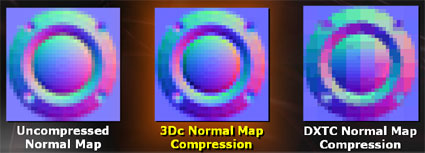
\includegraphics[width=0.60\columnwidth]{images/3dc_sample.jpg}%
	\caption{Compression d'une normal map par la compression 3Dc comparé à la compression DXT}%
	\label{}%
	\end{center}
\end{figure}

Les normal map comportent tout de même des inconvénients. D'une part, leur utilisation consiste à peu près à appliquer une texture au pixel, ce qui augmente la charge du CPU. D'autre part, le nombre de données nécessaires est plus grand car plus le développeur souhaite ajouté des détails, plus la résolution de la normal map doit être élevée et donc plus il faut de bande passante pour le chargement. 

Les compressions DXT et 3Dc permettent d'optimiser la vitesse de chargement des textures tout en ayant une qualité visuelle satisfaisante.

%------------------------------------------------
\newpage
\section{Remarque sur les shaders}
Le chargement du niveau peut être réduit en déportant les ressources graphiques dans les shaders. Par exemple, au lieu de charger le monde et les shaders, nous chargeons une représentation compressée du monde pour le générer par algorithme et nous gérons le texturage et l'affichage de celui ci via shader. 

Les shaders ayant une taille plus petite, ils sont de ce fait plus rapides à charger mais demandent plus de puissance coté GPU. Ainsi, nous pouvons afficher un terrain complexe avec de nombreux détails de profondeur et un texturage très différent en fonction de son niveau par rapport à la mer, en générant les différents changements dans le shader.

Il en va de même pour tous les effets liés à la météo, les godray, etc. Tous ces effets peuvent être codés et chargés rapidement dans un ensemble de shaders qui prennent peu de place en mémoire et sur le disque. Ainsi, il devient possible d'améliorer nettement les performances sur des supports beaucoup plus lents que les PC comme les consoles de salon et portables.

Pour généraliser cette idée, nous pouvons dire que s'il est possible d'effectuer un rendu par les shaders, le mettre en place sera forcément positif pour le chargement du jeu.

Les shaders étant compilés lors de leur utilisation pour s'adapter à la machine cible, il convient cependant de stocker une version de ceux ci dans un cache local pour ne pas avoir à les régénérer à chaque fois, ce qui aurait un effet contraire sur le chargement du jeu.

%------------------------------------------------
\newpage
\section{Optimisation par le level design}
\subsection{Conception du monde}
Une autre façon d'améliorer les temps de chargement est d'adapter le level design afin de satisfaire les exigences des plate formes visées. Par exemple, si nous prenons la carte d'un jeu à monde ouvert comme GTA 3, sorti sur PlayStation 2 et PC nous pouvons voir que les différentes parties de la ville sont organisées de façon à laisser un 'couloir' disponible pour que les chargements liés aux déplacements du joueur puissent avoir lieu.

\begin{figure}[!h]%
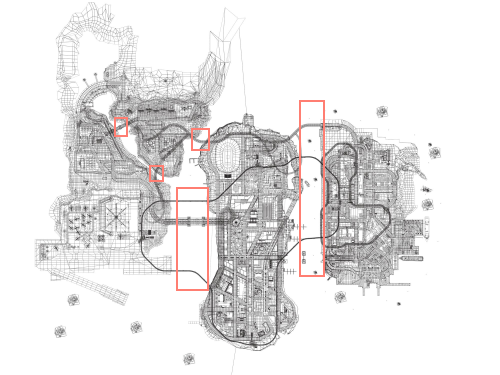
\includegraphics[width=\columnwidth]{images/gta3_map.png}%
\caption{Zones de chargement dans GTA 3}%
\label{}%
\end{figure}

Cependant, les chargements sont appliqués de manière assez brutale, le jeu étant bloqué en attendant la réception des données. Rockstar a donc échoué à proposer un chargement fluide malgré l'adaptation du level design, cependant cette technique leur a permis d'imposer un chargement dans des zones sans intérêt pour que le joueur puisse profiter d'un jeu fluide en dehors de ces zones tampons.

\newpage
\subsection{Intégration au monde}
Les chargements peuvent être intégrés au jeu et complètement transparents pour l'utilisateur. Si nous prenons l'exemple de Metroid Prime sur Gamecube, le jeu très détaillé nécessite de charger beaucoup de données. Cependant, il ne présente aucun écran de chargement. Les développeurs ont eu une idée astucieuse pour camoufler ces chargements et savoir dans quelle zone le joueur va se diriger pour charger uniquement le nécessaire.

\begin{wrapfigure}{l}{0.39\textwidth}
\begin{center}
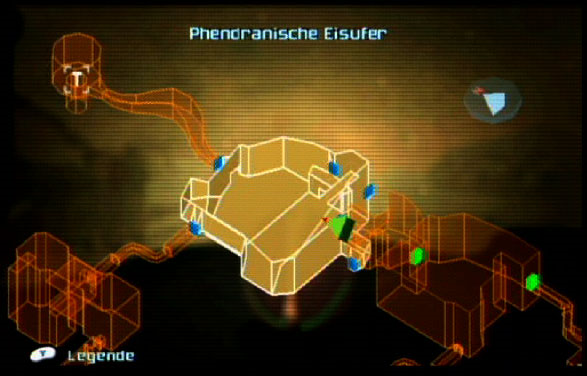
\includegraphics[width=0.38\textwidth]{images/metroid-prime_map.png}
\end{center}
\caption{Salle d'un niveau de Metroid Prime}
\end{wrapfigure}

Sur l'image ci-contre, nous pouvons apercevoir une salle d'un niveau du jeu, avec en bleu les portes qui permettent au joueur de quitter la salle pour en rejoindre une autre. A priori, impossible de savoir vers quelle porte le joueur va se diriger, et charger l'ensemble des zones connectées prendrait trop de mémoire et ne permettrait pas d'avoir un monde aussi détaillé. Pour résoudre ce problème, les développeurs du jeu ont trouvé une astuce: demander au joueur de réaliser une action vers la porte qu'il souhaite franchir, en tirant dessus. Une fois le tir envoyé sur la porte, le chargement de la zone connectée est lancé.

\begin{wrapfigure}{r}{0.35\textwidth}
\begin{center}
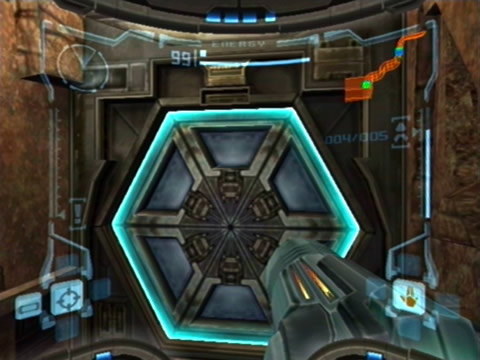
\includegraphics[width=0.33\textwidth]{images/metroid-prime_door.png}
\end{center}
\caption{Porte avant activation}
\end{wrapfigure}
Visuellement, le joueur comprend la situation: une porte bleue est une porte qui peut être ouverte avec un tir, et une fois que le halo bleu a disparu, la porte se prépare à être ouverte au bout d'un certain délai, plus ou moins long. Cependant le fait que l'utilisateur soit actif pour ces zones de chargement donne l'impression que le jeu n'en présente pas.

Ce mécanismes se retrouvent dans de nombreux autres jeux, où un obstacle nous fait face (souvent une porte ou un portail) et ne s'ouvre que lorsque la zone suivante est complètement chargée.
Dans un monde ouvert, cela peut poser un problème puisque cette méthode semble plus adaptée aux jeux découpés en salles. Cependant nous pouvons appliquer ce mécanismes aux habitations qui bordent les routes, aux grottes bloquées par un rocher à exploser, etc.


\newpage
\section{Apports du mémoire}
Le mémoire nous a permis d'en apprendre beaucoup plus sur les techniques de développement et de distribution des jeux vidéos. Plus que de simplement voir les techniques utilisées dans l'industrie, nous avons pu comprendre pourquoi les développeurs faisaient certains choix.

Ainsi, nous savons à présent comment nous y prendre au niveau du développement console passé et à venir, et comment organiser nos divers projets de jeux. Par exemple, nous comprenons pourquoi le jeu réalisé à l'ESGI l'année dernière sur PSP était soumis à des temps de chargements relativement longs, et nous pouvons maintenant les améliorer, voir les réduire à un niveau imperceptible par le joueur.

Ce sujet aborde un problème hautement technique mais assez méconnu, les joueurs et les développeurs étant souvent plus enclin à remarquer les prouesses graphiques ou liées au gameplay.

Cependant il s'agit d'un sujet vaste, et nous n'avons pu en explorer que la surface. Mais la connaissance de cette surface nous a permis d'avoir le minimum requis pour être indépendant dans nos recherches et nos développements, et nous donne la possibilité d'aborder notre propre façon de voir et de construire les projets que nous allons réaliser par la suite.

%------------------------------------------------

\newpage
\section{Conclusion}

Les jeux ont beaucoup évolués depuis leur création. Aujourd'hui, ils sont très volumineux car ils contiennent un nombre de ressources très élevé qui sont souvent réalisées en haute résolution afin d'obtenir une qualité visuelle importante. Il est donc judicieux de s'intéresser aux différentes techniques permettant de gérer au mieux ces ressources. Nous avons vu que de nombreux paramètres (tels que les composants physiques de la console ou de la machine, le support de stockage contenant les données du jeu, etc.) doivent être pris en compte pour choisir les techniques les plus efficaces à utiliser. 

Le but pour les développeurs est de réussir à optimiser le volume des données mais surtout les temps de chargement de celles-ci au cours d'une session de jeu. Il est intéressant de noter que les techniques d'optimisation sont très diverses et ne s'appliquent pas uniquement aux données du jeu. En effet, bien que la compression est une méthode très utilisée par les développeurs, il est possible d'optimiser le temps de chargement en organisant correctement les données sur le support de stockage. Il est même courant d'adapter le level design pour effectuer un chargement lorsque le joueur atteint une zone prédéfinie.

En général, le support de stockage, les consoles ou machines sur lesquelles doivent tourner les jeux sont fixés par les éditeurs et le marché actuel, les développeurs doivent s'adapter pour produire un jeu stable. Il s'agit donc pour eux de bien comprendre comment fonctionnent les différents composants de la machine tels que le disque dur, le lecteur de disque et le processeur. En effet, d'une machine à l'autre et selon le support de stockage utilisé il sera plus ou moins judicieux d'organiser les données de manière à ce qu'elles soient chargées les unes à la suite des autres pour éviter que le lecteur ait besoin d'effectuer un nouveau tour pour se repositionner.

En ce qui concerne la compression, elle est indispensable pour les jeux actuels. En effet, le volume de données peut atteindre 20 Go pour certains jeux les plus vendus et parfois plus. Même si les disques utilisés par les consoles possèdent une grosse capacité de stockage, il faut tout de même compresser les données afin de réduire leur poids et surtout pour augmenter la vitesse de chargement. Comme souvent, toute compression de données équivaut à une perte d'information et donc de qualité. Il faut alors savoir comment ajuster le taux de compression pour obtenir un bon rapport qualité/vitesse de transfert. Nous avons pu voir qu'il existe de nombreux formats de compression pour chaque type de données et que tous ont leurs avantages et leurs inconvénients. Par exemple, il est plus intéressant d'utiliser le format PNG plutôt que JPG pour les images, pour la compression de texture, il est possible d'utiliser les compressions DXT ou 3Dc, en sachant que les textures de type normal map seront de meilleure qualité avec la compression 3Dc.

Nous avons aussi constaté que les développeurs utilisent parfois directement le level design pour permettre un chargement en tâche de fond en fonction des actions du joueur. Dans le jeu Dead Space, certaines portes s'ouvrent au bout d'un certain temps. Il s'agit d'une technique basée sur celle du jeu Resident Evil où une animation est lancée à chaque fois que le joueur ouvre une porte. Cette méthode permet en quelque sorte de créer l'illusion qu'il n'y a aucun chargement.

Il est intéressant de constater que l'accumulation de toutes ces techniques permet d'optimiser au maximum le jeu final tout en conservant sa qualité visuelle. Ces techniques peuvent être difficiles à mettre en place mais elles sont indispensables pour de gros jeux possédant une quantité impressionnante de données. Ces méthodes sont aussi conseillées pour des jeux moins ambitieux en terme de contenu.

A force d'améliorer ou de créer de nouvelles techniques d'optimisation, les jeux actuels possèdent peu de temps de chargement ce qui est un atout majeur pour la fluidité et le dynamisme. Puisque les jeux vidéo et la nouvelle technologie évoluent d'année en année, nous pouvons espérer que dans un futur proche, la vitesse de transfert des données sera tellement rapide que le chargement deviendra invisible et donc inexistant aux yeux des joueurs.

%----------------------------------------------------------------------------------------
%	BIBLIOGRAPHY
%----------------------------------------------------------------------------------------
\newpage
\bibliographystyle{unsrt}
\bibliography{References}

%----------------------------------------------------------------------------------------

\end{document}
